
\bigskip
\noindent
The fundamental theorem of calculus
is a formal expression of the inverse relation between
integrals and derivatives.
$$\int_a^b f'(x)\,dx=f(b)-f(a)$$
Here is an Eigenmath demonstration of the fundamental theorem of calculus.

\begin{Verbatim}[formatcom=\color{blue},samepage=true]
xrange = (-1,1)
yrange = (-1,1)
f = d(x^2/2)
draw(f,x)
\end{Verbatim}

\begin{center}
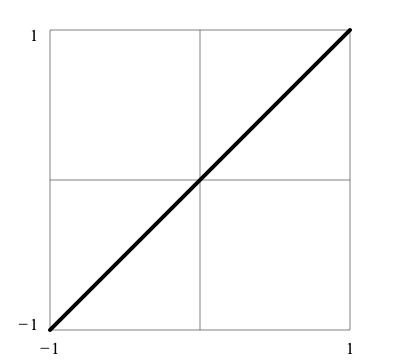
\includegraphics[scale=0.5]{funda1.png}
\end{center}

\begin{Verbatim}[formatcom=\color{blue},samepage=true]
xrange = (-1,1)
yrange = (-1,1)
f = integral(d(x^2/2))
draw(f,x)
\end{Verbatim}

\begin{center}
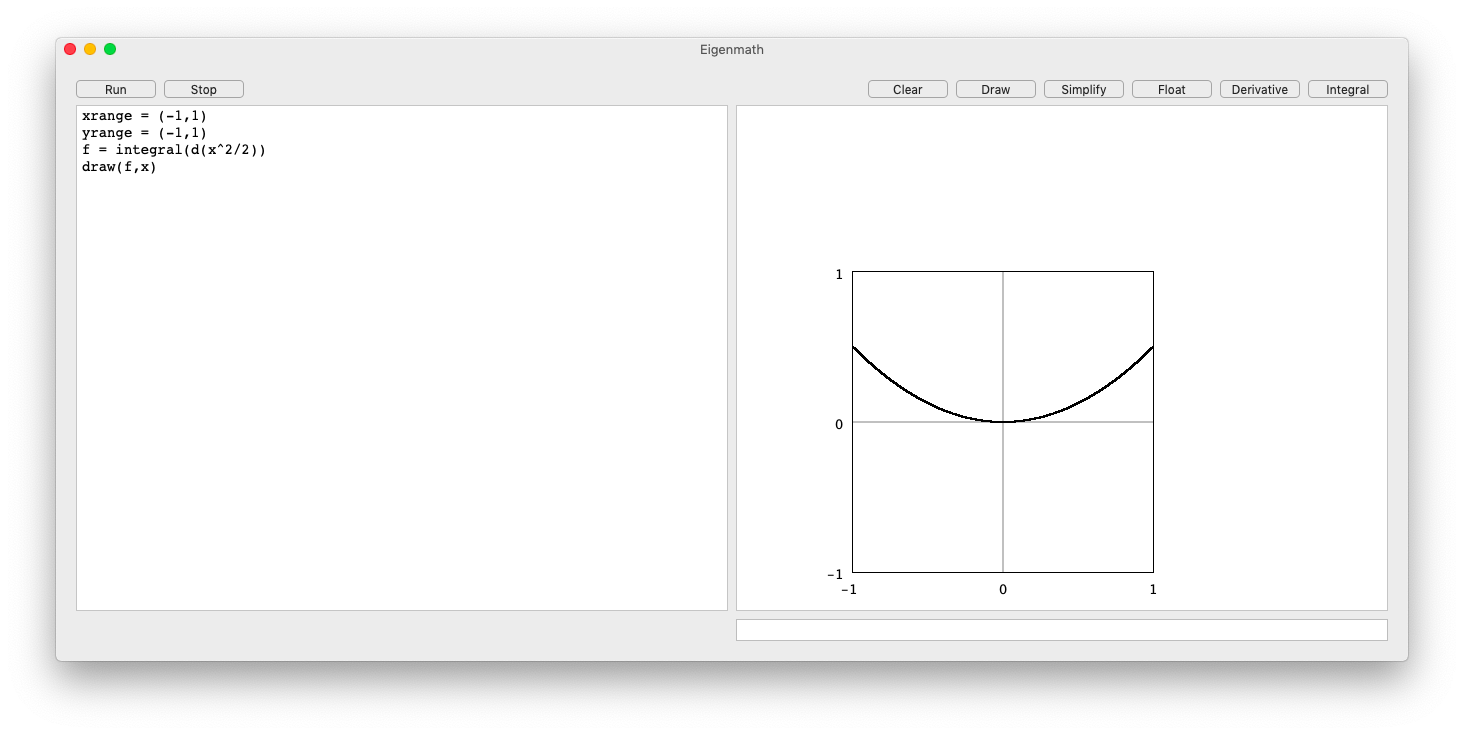
\includegraphics[scale=0.5]{funda2.png}
\end{center}

\noindent
The first graph shows that $f'(x)$ is antisymmetric, therefore the total
area under the curve from $-1$ to $1$ sums to zero.
The second graph shows that $f(1)=f(-1)$.
Hence for $f(x)=\tfrac{1}{2}x^2$ we have
$$\int_{-1}^1f'(x)\,dx=f(1)-f(-1)=0$$
